\documentclass[11pt]{beamer}
\usetheme{Frankfurt}
\usepackage[utf8]{inputenc}
\usepackage{amsmath}
\usepackage{amsfonts}
\usepackage{amssymb}
\usepackage{subcaption}
\usepackage[export]{adjustbox}

\setbeamercolor{emph}{fg=blue}
\renewcommand<>{\emph}[1]{%
  {\usebeamercolor[fg]{emph}\only#2{\itshape}#1}%
}
%-------------------------------------------------------------------------
\author{Florencia Zanollo}
\title{Analysis of anime voice actor's social network and popularity}
%\setbeamercovered{transparent} 
%\setbeamertemplate{navigation symbols}{} 
%\logo{} 
\institute{University of Buenos Aires (Argentina) - National Institute of Informatics (Japan)} 
\date{} 
%\subject{} 
%-------------------------------------------------------------------------
\begin{document}

\begin{frame}
\titlepage
\end{frame}

\begin{frame}
\tableofcontents
\end{frame}

%-------------------------------------------------------------------------
\section{Introduction}
\begin{frame}{Introduction}

Our research went through multiple stages. Starting with Linked Open Data, moving to Social Network Analysis and ending with applied machine learning.
\vspace{15pt}

Thus the order of this presentation will be chronological.
\vspace{15pt}

Nonetheless our main focus is: \emph{Social network of seiyuu} (or anime's voice actors)
\end{frame}
%-------------------------------------------------------------------------
\section{Dataset}
\subsection{Why seiyuu?}
\begin{frame}{Why seiyuu?}
\begin{itemize}
\item Because I \textbf{really} like anime and manga.

\item There are many researches whose focus is actor's social network but usually is hollywood actors and not only voice actors. Seiyuu and anime industry is really unusual and so could present a different structure.

\item There're several database with information about anime and seiyuu but either it's incomplete or doesn't have a good structure nor format.
\end{itemize}
\end{frame}
%-------------------------------------------------------------------------

\subsection{Wikidata and MyAnimeList}
\begin{frame}{Wikidata and MyAnimeList}
We wanted to use \emph{Wikidata} as our source but it's too incomplete; it doesn't have information about works of seiyuu.
\vspace{15pt}

Instead we used \emph{MyAnimeList} (MAL) through an API called \emph{Jikan}; retrieving data in JSON and then changing its format to RDF.
\vspace{15pt}

We used Wikidata to get the list of seiyuu and MyAnimeList to get list of works for each seiyuu and information about anime.
\end{frame}
%-------------------------------------------------------------------------

\begin{frame}
\begin{center}
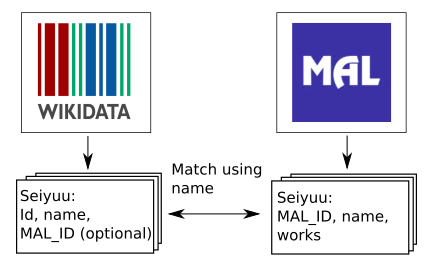
\includegraphics[scale=0.7]{graphics/wikidataMAL.png} 
\end{center}

\begin{itemize}
\item Total of 6472 seiyuu on Wikidata
%There’s actually 7030 seiyuu in wikidata but only 6472 of them have an English label
\item Only 59 had MAL\_IDs
\item 3033 MAL\_IDs retrieved
\item At the end having 3092 seiyuu with MAL\_ID
\item 2956 of which had at least one work

\end{itemize}
\end{frame}
%-------------------------------------------------------------------------

\subsection{Data retrieved}
\begin{frame}{Data retrieved}
All in all we were able to retrieve the following information for \emph{2956 seiyuu and 7614 anime}.

\begin{itemize}
	\item For Seiyuu:
	\begin{itemize}
		\item Name
		\item Debut (this was obtained from oldest work's aired date)
		\item Gender
		\item Popularity (member\_favorites information of MAL)
		\item Works (anime roles with anime information plus wheter is a main role or not)
	\end{itemize}
	\item For Works (Anime):
	\begin{itemize}
		\item Year that began airing
		\item Favorites
		\item Score (from 0 to 10, MAL user based)
		\item Popularity (ranking over all MAL animes)
		\item Members (how many MAL users have it on their list)
		\item Genres
	\end{itemize}
\end{itemize}
\end{frame}
%-------------------------------------------------------------------------
\section{Social Network}
\subsection{Construction}
\begin{frame}{Social Network}
This social network is of a particular kind called \emph{two-mode networks} which consists of a set of actors (seiyuu) and events (anime).
\vspace{15pt}

Details to consider:
\begin{itemize}
\item We can choose between anime and seiyuu as nodes.
\item Nodes are time dependant (since they have debut year).
\item Edge or relationship definition:
	\begin{itemize}
	\item How many works in common?
	\item Which time frame?
	\end{itemize}
\end{itemize}
\vspace{15pt}
\end{frame}
%-------------------------------------------------------------------------

\begin{frame}
We compared two graph definitions using \emph{seiyuu as nodes} and, as edge definition:
\begin{itemize}
\item at least 1 work in common
\item at least 10 works in common
\end{itemize}
Both of them during the time frame between the first debut registered (1960) and the year of observation.
\end{frame}
%-------------------------------------------------------------------------

\subsection{Analysis}
\begin{frame}{One work in common}
\begin{figure}
	\begin{subfigure}{.6\linewidth}
		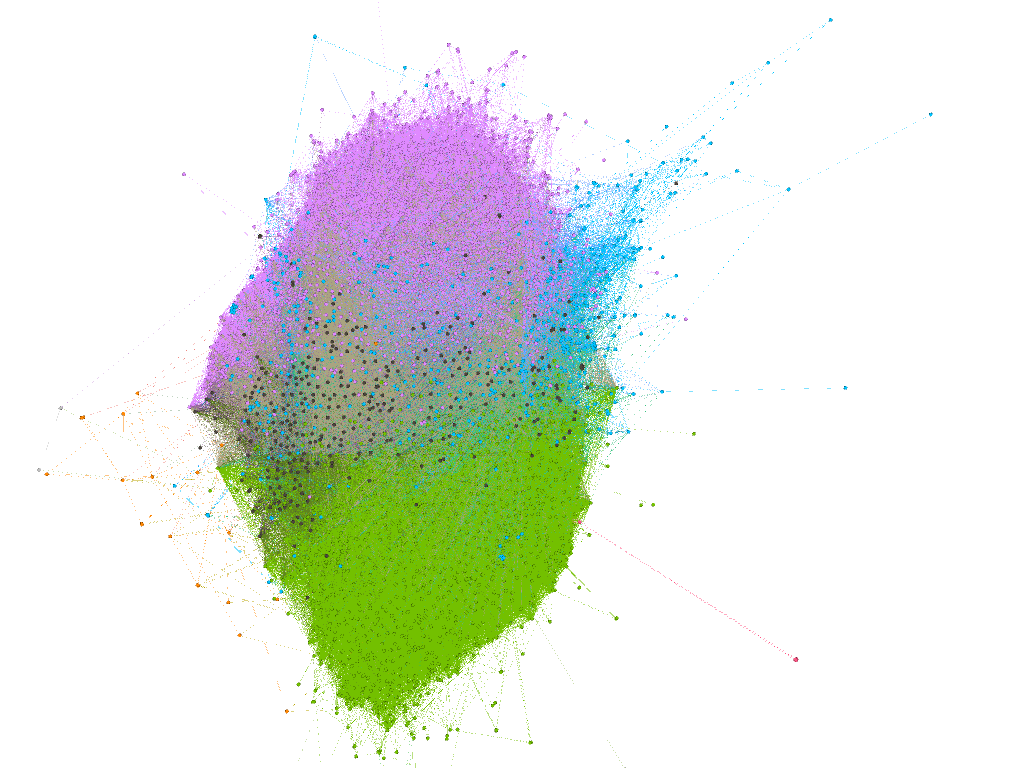
\includegraphics[scale=0.27, left]{graphics/atLeast1WorkCommunity.png} 
	\end{subfigure}%
	\begin{subfigure}{.4\linewidth}
		\begin{description}
		\item[Avg degree] 267
		\item[Graph density] 0.09
		\item[Modularity] 0.2
		\item[Network diameter] 6
		\item[Connected components] 18
		\end{description}
	\end{subfigure}
\end{figure}
\end{frame}
%-------------------------------------------------------------------------

\begin{frame}{Ten works in common}
\begin{figure}
	\begin{subfigure}{.55\linewidth}
		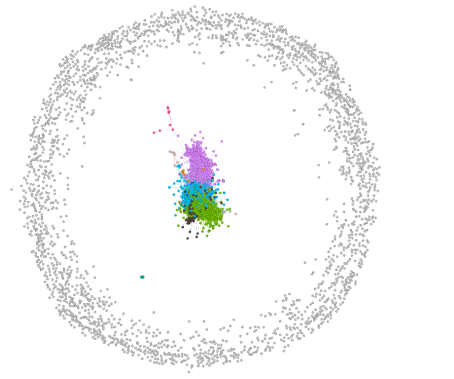
\includegraphics[scale=0.55, left]{graphics/atLeast10WorksCommunity.png} 
	\end{subfigure}%
	\begin{subfigure}{.45\linewidth}
		\begin{description}
		\item[Avg degree] 9
		\item[Graph density] 0.003
		\item[Modularity] 0.29
		\item[Network diameter] 7
		\item[Connected components] 2261
		\end{description}
	\end{subfigure}
\end{figure}
\end{frame}
%-------------------------------------------------------------------------

\begin{frame}{Features}
\begin{description}
	\item [Strongly connected] With merely $\sim$3000 nodes it has $\sim$400000 edges when only one work in common is required and $\sim$14000 edges when asking for 10 or more. 
	\item [Big cluster] Thightly interconnected and big cluster surrounded by poorly or not connected nodes. (99\% of the nodes of one work in common graph and 23\% of 10 works in common). 
	\item [Communities] We can see at least four clear communities in each graph.
	\item [Nodes] This graph is accumulative, so long carrier almost always means a strong node.
\end{description}
\end{frame}
%-------------------------------------------------------------------------

\begin{frame}{Edge growth}
\begin{figure}
	\centering
	\begin{subfigure}{.5\columnwidth}
		\centering
		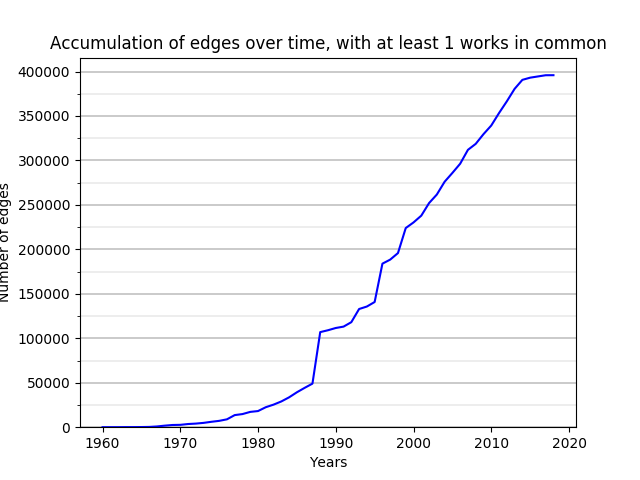
\includegraphics[scale=0.35]{graphics/accumulationEdges_1_1960-2018.png}
	\end{subfigure}%
	\begin{subfigure}{.5\columnwidth}
		\centering
		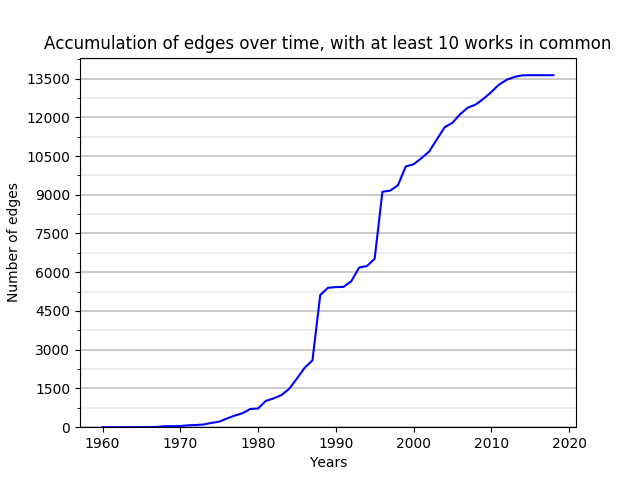
\includegraphics[scale=0.35]{graphics/accumulationEdges_10_1960-2018.png}
	\end{subfigure}
\end{figure}
\begin{itemize}
\item Edge growth follows the same distribution with 1 and 10 works in common
\end{itemize}
\end{frame}
%-------------------------------------------------------------------------

\begin{frame}{Node growth}
\begin{center}
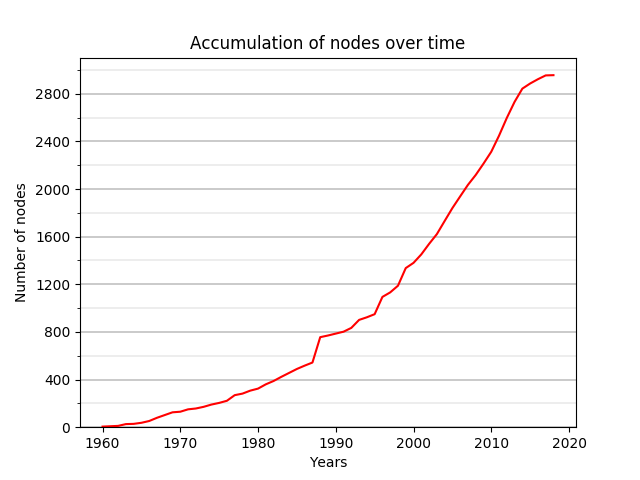
\includegraphics[scale=0.5]{graphics/nodesAccumulation.png} 
\end{center}
\begin{itemize}
\item More than half of the nodes are from last 18 years (2000 to 2018)
\end{itemize}
\end{frame}
%-------------------------------------------------------------------------

\begin{frame}{Top 5 degree}
\begin{table}[!htb]
    \begin{minipage}{.5\textwidth}
        \centering
            \begin{tabular}{|l|c|}
				\hline
				Name & Degree \\ 
				\hline
				Takehito Koyasu & 1545 \\ 
				\hline
				Akira Ishida & 1488 \\ 
				\hline
				Mamiko Noto & 1422 \\ 
				\hline
				Nobuo Tobita & 1417 \\ 
				\hline
				Daisuke Namikawa & 1390 \\ 
				\hline
			\end{tabular}
            \caption{One work in common}
    \end{minipage}%
    \begin{minipage}{.6\textwidth}
        \centering
        \begin{tabular}{|l|c|}
				\hline
				Name & Degree \\
				\hline
				Takehito Koyasu & 311 \\
				\hline
				Akira Ishida & 273 \\
				\hline
				Mamiko Noto & 258 \\
				\hline
				Daisuke Namikawa & 232 \\
				\hline
				Katsuyuki Konishi & 229 \\
				\hline
			\end{tabular}
            \caption{Ten works in common}
    \end{minipage}
\end{table}
\end{frame}
%-------------------------------------------------------------------------

\begin{frame}{Top 5 betweenness centrality}
\begin{table}[!htb]
    \begin{minipage}{.5\textwidth}
        \centering
            \begin{tabular}{|l|c|}
				\hline
				Name & BtwC \\
				\hline
				Takehito Koyasu & 49982.52 \\
				\hline
				Akira Ishida & 40221.50 \\
				\hline
				Daisuke Namikawa & 30448.43 \\
				\hline
				Nobuo Tobita & 29363.25 \\
				\hline
				Mamiko Noto & 29168.18 \\
				\hline
		\end{tabular}
        \caption{One work in common}
    \end{minipage}%
    \begin{minipage}{.5\textwidth}
        \centering
        \begin{tabular}{|l|c|}
				\hline
				Name & BtwC \\
				\hline
				Takehito Koyasu & 18489.44 \\
				\hline
				Mamiko Noto & 10988.96 \\
				\hline
				Daisuke Namikawa & 9570.48 \\
				\hline
				Akira Ishida & 8299.19 \\
				\hline
				Rie Kugimiya & 7560.16 \\
				\hline
		\end{tabular}
        \caption{Ten works in common}
    \end{minipage}
\end{table}
\end{frame}
%-------------------------------------------------------------------------

\begin{frame}
Both networks have fairly similar top 5s so it points to them having similar structure and connections amoung their nodes, aside from actual values.
\vspace{10pt}

From now on our graph definition will be:
\begin{description}
\item[Node] Seiyuu
\item[Edge] At least 10 works in common from 1960 to year of observation.
\end{description}
\vspace{10pt}

Because requiring more jobs in common means less amount of edges, this leaves a more understandable graph and we verified it does without changing its structure so much.
\end{frame}
%-------------------------------------------------------------------------
\section{Popularity}
\subsection{Definition}
\begin{frame}{Popularity: Definition}
Since we are using MAL database and it has a social component, seems logic to use \emph{member\_favorites} as a representation of \emph{popularity}. We can also get popularity and score of anime from opinions of the same set of users.
\vspace{-10pt}

\begin{table}[!h]
	\begin{center}
	\begin{tabular}{|l|c|l|}
		\hline
		Name & Popularity & Some popular roles of them\\ 
		\hline
		Kana Hanazawa & 56637 & \textit{Angel Beats!}: Tachibana, Kanade \\
		\hline
		Hiroshi Kamiya & 49685 & \textit{Shingeki no Kyojin}: Levi, \\
		\hline
		Mamoru Miyano & 43942 & \textit{Death Note}: Yagami, Light \\ 
		\hline
		Rie Kugimiya & 31668 & \textit{Fullmetal Alchemist}: Elric, Alphonse \\ 
		\hline
		Jun Fukuyama & 26811 & \textit{Ao no Exorcist}: Okumura, Yukio \\ 
		\hline
		Miyuki Sawashiro & 26501 & \textit{Durarara!!}: Sturluson, Celty \\ 
		\hline
		Tomokazu Sugita & 24449 & \textit{Gintama}: Sakata, Gintoki \\
		\hline
		Daisuke Ono & 24080 & \textit{Durarara!!}: Heiwajima, Shizuo \\
		\hline
		Saori Hayami & 18322 & \textit{Owari no Seraph}: Hiiragi, Shinoa \\ 
		\hline
		Aya Hirano & 18094 & \textit{Fairy Tail}: Heartfilia, Lucy \\
		\hline
	\end{tabular}
	\end{center}
\end{table}
\end{frame}
%-------------------------------------------------------------------------

\subsection{Analysis}
\begin{frame}{Popularity: Analysis}
\begin{center}
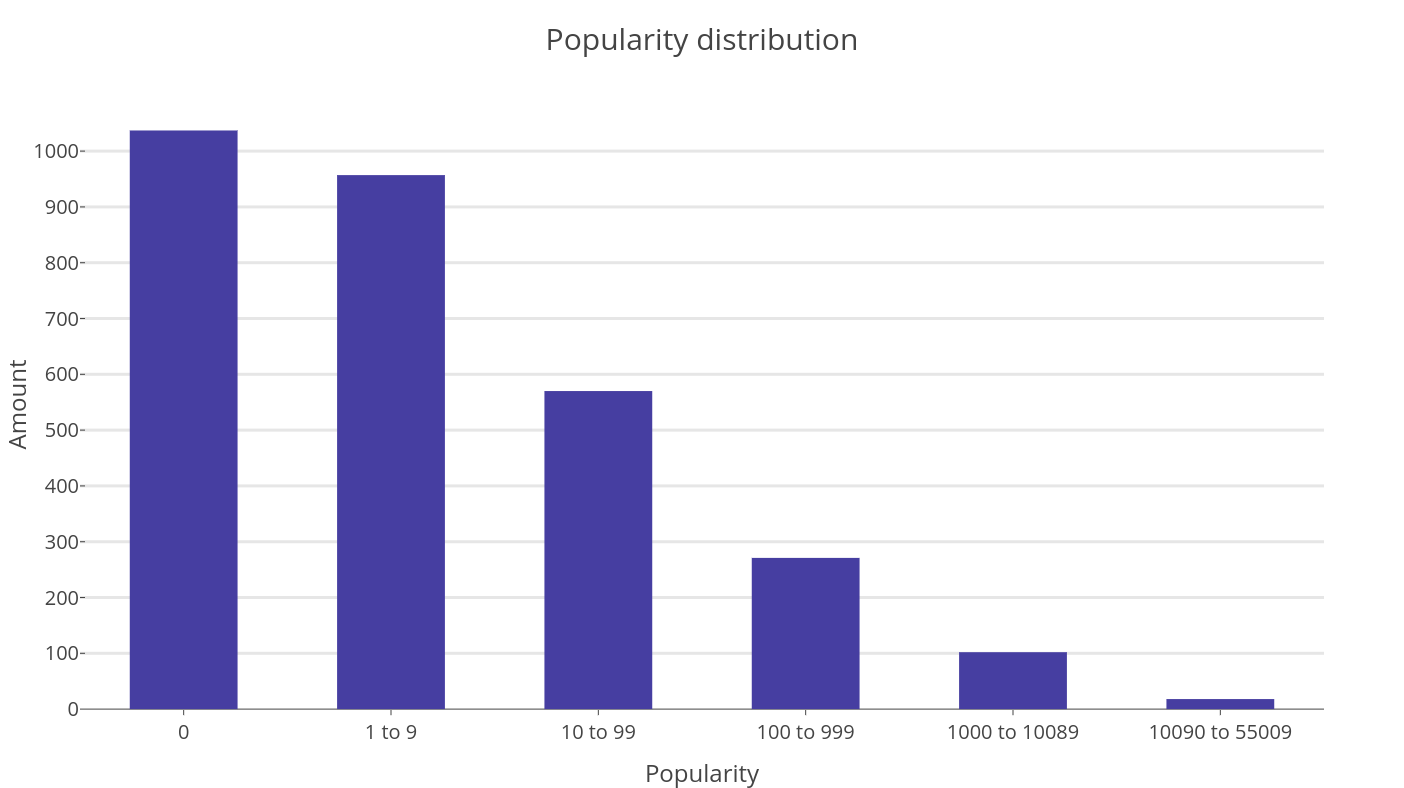
\includegraphics[scale=0.2]{graphics/popularityDistribution.png} 
\end{center}
\begin{table}[!htb]
    \begin{minipage}{.4\textwidth}
		\begin{itemize}
	\item Total: 2956
	\item Mean:    289.55
	\item Median:    2.0
		\end{itemize}
    \end{minipage}%
    \begin{minipage}{.6\textwidth}
        	\begin{itemize}
	\item Min:    0; Max:    55018
	\item 1037 values equal to zero
	\item Only 120 values bigger than 1000
		\end{itemize}
    \end{minipage}
\end{table}
\end{frame}
%-------------------------------------------------------------------------

\subsection{Pearson correlation}
\begin{frame}{Popularity: Pearson correlation}
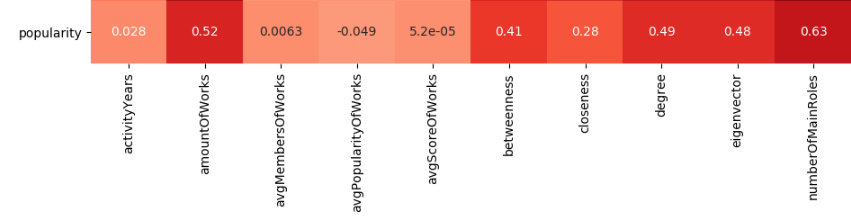
\includegraphics[scale=0.45]{graphics/popCorrelationAllWorks.png} 
\begin{itemize}
\item Big correlation between popularity and amount of works. %This attribute doesn't have the biggest correlation with popularity but "number of main roles" was added to the end of this investigation since we didn't had the data for doing so before. 
\item Number of main roles and amount of works have a strong correlation with each other (0.9) but they have different influence over popularity, this means they provide distinct information.
\end{itemize}

\end{frame}
%-------------------------------------------------------------------------

\begin{frame}
Since our dataset is biased in favor of more modern anime we thought of correlate with \emph{recent works} only.
\vspace{5pt}

But, how recent? Last 5, 10 or 20 years? 
\vspace{-5pt}

\begin{center}
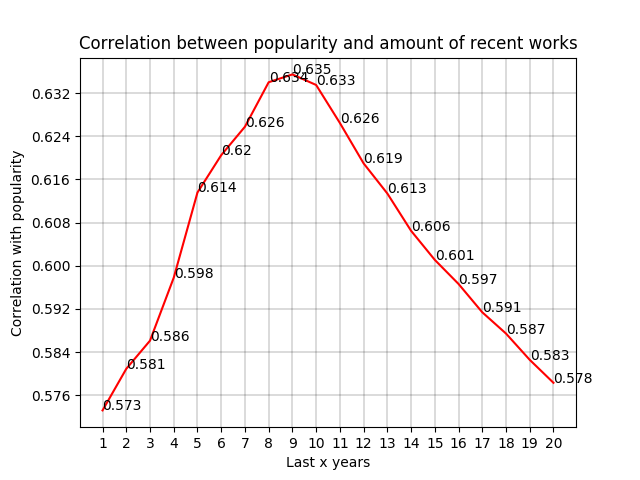
\includegraphics[scale=0.6]{graphics/correlationPopRecentWorks.png} 
\end{center}

\end{frame}
%-------------------------------------------------------------------------

\begin{frame}
So our definition of \emph{recent works} will be \emph{last 9 years}.
\begin{center}
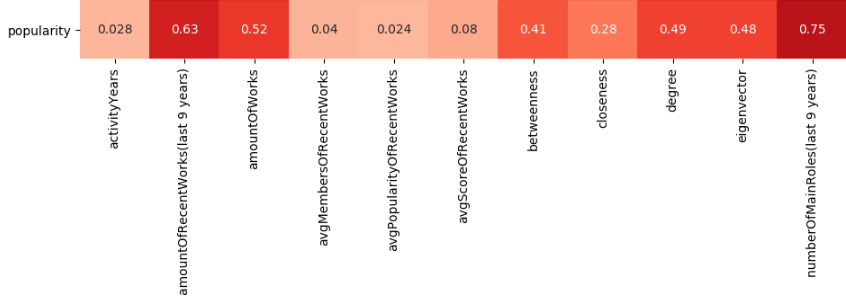
\includegraphics[scale=0.45]{graphics/popCorrelationRecentWorks.png} 
\end{center}
\begin{itemize}
\item Amount of recent works has more correlation with popularity than not recent.
\item It also happens with number of main roles.
\end{itemize}
\end{frame}
%-------------------------------------------------------------------------

\begin{frame}
Next graphs were made in order to discover \emph{why} \textit{9 years} prior had more correlation. 
\vspace{-5pt}
\begin{figure}
	\centering
	\begin{subfigure}{.45\columnwidth}
		\centering
		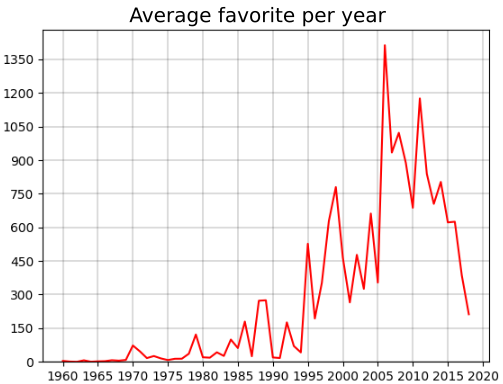
\includegraphics[width=\columnwidth]{graphics/avgFavorites.png}
	\end{subfigure}%
	\begin{subfigure}{.45\columnwidth}
		\centering
		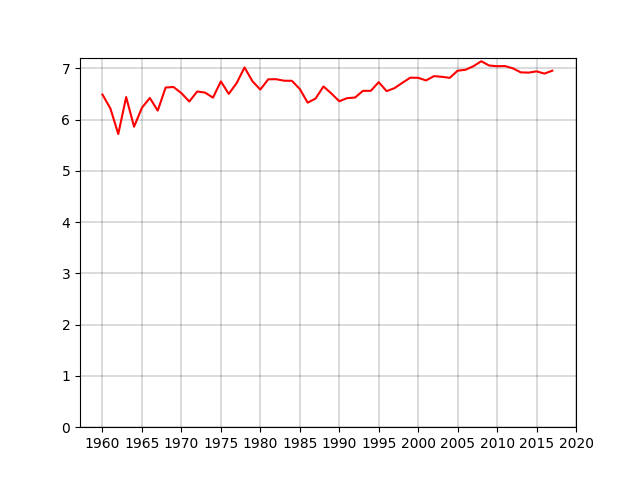
\includegraphics[width=\columnwidth]{graphics/avgScores.png}
	\end{subfigure}
	\begin{subfigure}{.45\columnwidth}
		\centering
		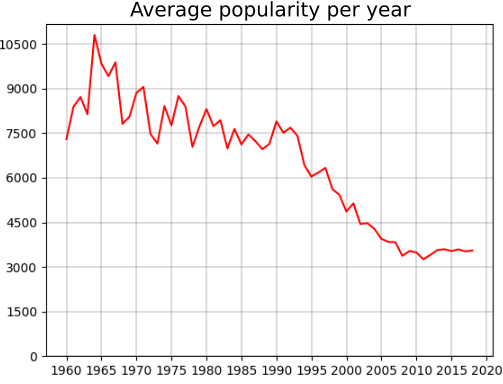
\includegraphics[width=\columnwidth]{graphics/avgPopularities.png}
	\end{subfigure}%
	\begin{subfigure}{.45\columnwidth}
		\centering
		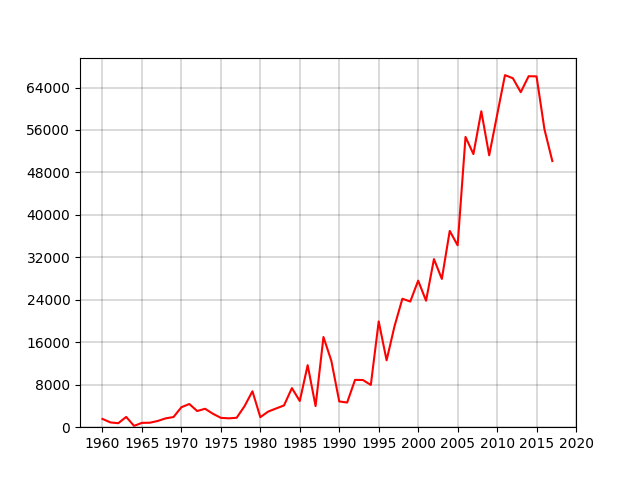
\includegraphics[width=\columnwidth]{graphics/avgMembers.png}
	\end{subfigure}
\end{figure}
\end{frame}
%-------------------------------------------------------------------------

\subsection{Prediction}
\begin{frame}{Popularity: Prediction}
The node attributes were divided into categories, leaving four distinct types:

\begin{figure}
	\centering
	\begin{subfigure}{.4\columnwidth}
		\begin{itemize}
			\item Personal data:
			\begin{itemize}
				\item Debut
				\item Gender
				\item Activity years (2018-debut)
			\end{itemize}
			\item Works data:
			\begin{itemize}
				\item Amount
				\item Top 5 genre
				\item Favorites
				\item Score
				\item Popularity
				\item Members
				\item Number of main roles
			\end{itemize}
		\end{itemize}
	\end{subfigure}%
	\begin{subfigure}{.6\columnwidth}
		\begin{itemize}
			\item Recent works data:
			\begin{itemize}
				\item Same as works but for only last 9 years
			\end{itemize}	
			\item Graph data:
			\begin{itemize}
				\item Degree
				\item Betweenness centrality
				\item Closeness
			\end{itemize}
		\end{itemize}
	\end{subfigure}
\end{figure}
\end{frame}
%-------------------------------------------------------------------------

\begin{frame}
Fitting and prediction experiments were run for each category, each combination of 2, 3 and all of them together; using Scikit-learn, 80\% of seiyuu as train data and the rest as test. This was done for all following models:
\begin{itemize}
	\item DecisionTreeRegressor
	\item DecisionTreeClassifier
	\item LinearRegression
	\item KNeighborsClassifier
	\item LinearDiscriminantAnalysis
	\item GaussianNB
	\item SVM
\end{itemize}
\end{frame}
%-------------------------------------------------------------------------

\begin{frame}
Because popularity variance is really high we got good results in metrics but particular predictions were aloof.
\vspace{5pt}

For example:\\
\emph{DecisionTreeClassifier} gets a r2\_score of 0.57 when using model data from \emph{works and recent works} categories but the scatter plot doesn't show such good results.
\vspace{-15pt}

\begin{figure}
	\begin{subfigure}{.5\columnwidth}
		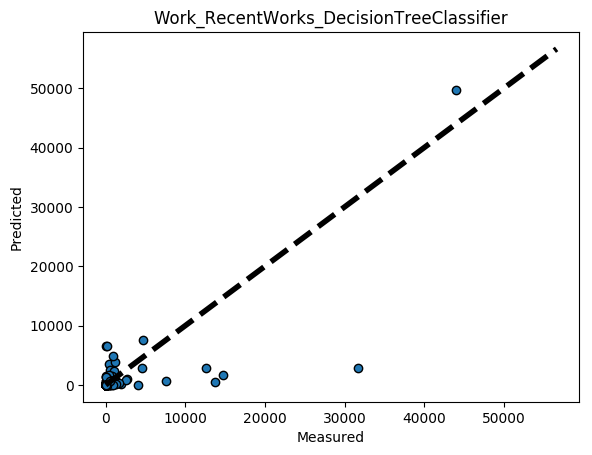
\includegraphics[scale=.36]{graphics/Work_RecentWorks_DecisionTreeClassifier.png} 
	\end{subfigure}%
	\begin{subfigure}{.5\columnwidth}
		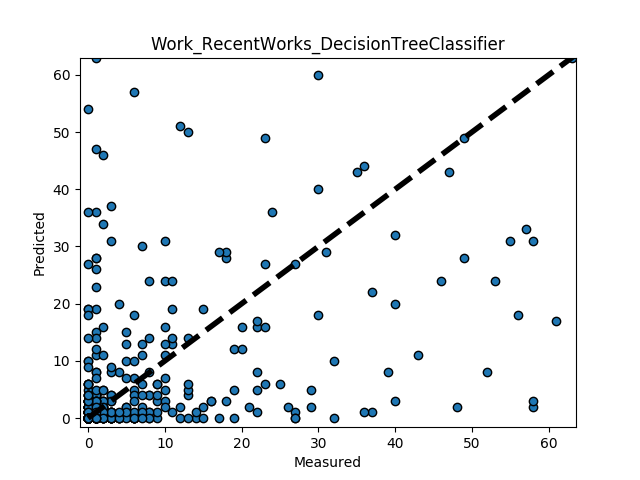
\includegraphics[scale=.4]{graphics/Work_RecentWorks_DecisionTreeClassifierZOOM.png} 
		\caption{Zoomed in}
	\end{subfigure}
\end{figure}

\end{frame}
%-------------------------------------------------------------------------

\begin{frame}{Popularity: Feature importance}
One of our goals about predicting popularity was to use the classifier algorithms to understand which are the key features that differentiates between a "not so much" and a popular seiyuu.
\vspace{5pt}

For our previous example we got:
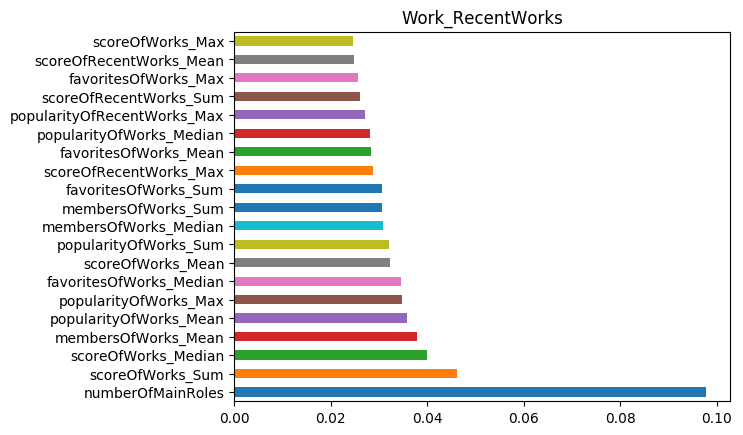
\includegraphics[scale=.5]{graphics/Work_RecentWorks_DTC_featureImportances.png} 

\end{frame}
%-------------------------------------------------------------------------
%-------------------------------------------------------------------------
\section{Conclusion}
\begin{frame}
conclusion
\end{frame}
%-------------------------------------------------------------------------
\end{document}